\documentclass[conference]{IEEEtran}
\IEEEoverridecommandlockouts
% The preceding line is only needed to identify funding in the first footnote. If that is unneeded, please comment it out.
\usepackage{cite}
\usepackage{amsmath,amssymb,amsfonts}
\usepackage{algorithmic}
\usepackage{orcidlink} 
\usepackage{graphicx}
\usepackage{textcomp}
\usepackage{xcolor}
\usepackage{subfigure}
\usepackage{orcidlink}
\usepackage{array}
\usepackage{gensymb}
\hypersetup{
    hidelinks,
}
\def\BibTeX{{\rm B\kern-.05em{\sc i\kern-.025em b}\kern-.08em
    T\kern-.1667em\lower.7ex\hbox{E}\kern-.125emX}}
\begin{document}

\title{Model-Driven Design Exploration of Hybrid Voltage Regulators for Vertical Power Delivery\\
\thanks{This work was supported by the Center for Heterogeneous Integration of Micro Electronic Systems (CHIMES), one of seven centers in Joint University Microelectronics Program (JUMP) 2.0, a Semiconductor Research Corporation (SRC) program sponsored by the Defense Advance Research Project Agency (DARPA).}
}


\author{
\begin{minipage}[t]{\linewidth}
    \centering
    Salma Abdelzaher\,\orcidlink{0009-0003-7242-5665},\;
    Mohamed Gharib\,\orcidlink{0009-0008-3606-6200},\;
    Inna Partin-Vaisband\,\orcidlink{0000-0002-6399-6672} \\
    University of Illinois Chicago, Chicago IL, USA \\
    sabdel29@uic.edu, mghari5@uic.edu, vaisband@uic.edu
\end{minipage}
\hfill
}

% \and
% \IEEEauthorblockN{5\textsuperscript{th} Given Name Surname}
% \IEEEauthorblockA{\textit{dept. name of organization (of Aff.)} \\
% \textit{name of organization (of Aff.)}\\
% City, Country \\
% email address or ORCID}
% \and
% \IEEEauthorblockN{6\textsuperscript{th} Given Name Surname}
% \IEEEauthorblockA{\textit{dept. name of organization (of Aff.)} \\
% \textit{name of organization (of Aff.)}\\
% City, Country \\
% email address or ORCID}

\maketitle

\begin{abstract}

Point-of-load power conversion for AI accelerators is no longer a single-converter problem---it is a coupled topology, device, passive,
switching frequency, and packaging co-optimization that cannot be
tractably solved by manual design. A model-driven framework for
series-capacitor buck hybrid voltage regulators (SC-Buck HVRs) is
proposed. Given user-specified conversion ratio, load current,
current density target, and package model, the framework enumerates all feasible
multi-phase architectures and co-optimizes devices, passives, and
switching frequency over real component libraries via a closed-form
loss model. Ripple, saturation, voltage-rating, and
area constraints are enforced throughout the optimization. The framework is validated against
Cadence Virtuoso/Spectre-designed SOTA topologies at
\textbf{95.27\,$\pm$\,1\%} loss prediction accuracy. Up to
\textbf{+4.6~pp} efficiency improvement and \textbf{29.2$\times$}
footprint reduction over SOTA baselines are demonstrated at identical
topology. 
Packaging-aware design-space exploration demonstrates that the optimal converter topology and component selections vary significantly across package implementations, highlighting the necessity of package-aware optimization.


\end{abstract}

\begin{IEEEkeywords}
High performance computing (HPC), AI Data Centers, power integrity, High-Step Voltage Regulation, Vertical Power Delivery, Buck Regulators.
\end{IEEEkeywords}

\section{Introduction}
The growing demand for AI workloads has driven next-generation accelerators beyond 1~kW per chip at sub-1~V supply rails. Concurrently, the industry-wide transition to 48~V intermediate-bus architectures imposes a severe 48:1 voltage conversion challenge at the point-of-load (POL)~\cite{Sri_SOCC,ECTCSalma26, EPEPS}. As shown in Fig.~\ref{current density spec}, POL current density has grown from 0.37~A/mm$^2$ in 2017 to over 1.2~A/mm$^2$ in 2025, requiring voltage regulator capable of sustaining $>$1~A/mm$^2$.% within tightly constrained footprints beneath the processor die.

Conventional single-stage topologies cannot meet this challenge.
Buck-only converters suffer an effective duty cycle of ${\sim}2\%$ at 48:1, rendering gate-driver timing margins impractical, while switched-capacitor (SC)-only converters
incur excessive hard-switching losses~\cite{comparison_SCbuck_and_buck}. 
Hybrid voltage regulators (HVRs), combining an SC front-end with a multiphase buck stage, reduce the input voltage to $V_\mathrm{in}/N$, extending the effective duty cycle by a factor of $N$ while
reducing switch stress to $V_\mathrm{in}/N$. The buck stage enables near-zero-voltage
turn-on of the low-side switches, substantially reducing switching losses~\cite{DPMIH44, DSCH, DSCB, DPMIH62}.

\begin{figure}[t]
    \centering
    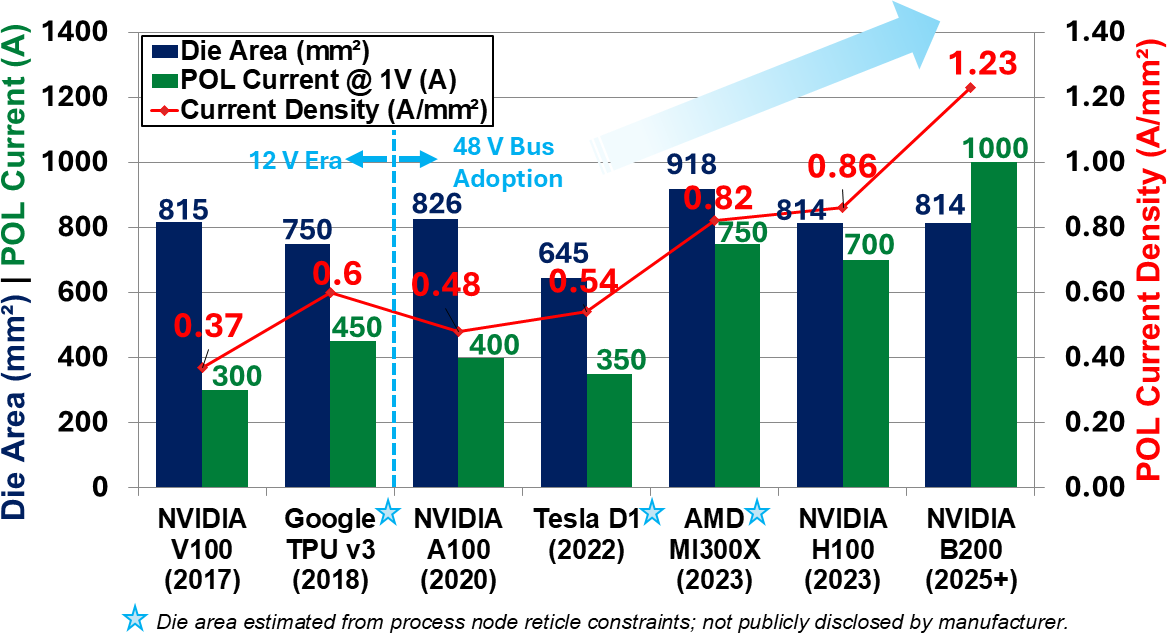
\includegraphics[width=0.46\textwidth]{CurrentDensity.png}
    \vspace{-5pt}
    \caption{AI accelerator scaling: die area, POL Current, and current density.}
    \vspace{-15pt}
    \label{current density spec}
\end{figure}


Despite demonstrated HVR implementations~\cite{DPMIH44, DSCH, DSCB, DPMIH62}, no systematic framework exists for joint topology and component
co-optimization---a combinatorial problem that is intractable to solve manually,
because practical devices are selected from discrete libraries rather than continuously sized. A model-driven framework is presented that enumerates all feasible
SC-buck architectures under user-defined constraints and co-optimizes
devices, passives, and switching frequency while enforcing ripple, saturation, and voltage-rating constraints. Validated against Cadence Virtuoso/Spectre simulations, the framework
recovers substantial efficiency and footprint improvements over manually designed state-of-the-art (SOTA). Packaging-aware design space exploration (DSE) further demonstrates that the optimal converter topology depends strongly on the integration scheme.

%The framework is presented in Section~II. Results are reported in Section~III. The paper is concluded in Section~IV.





\section{Proposed Framework}
\label{HVR Architecture and Loss Model}

\begin{figure}[t]
    \centering
    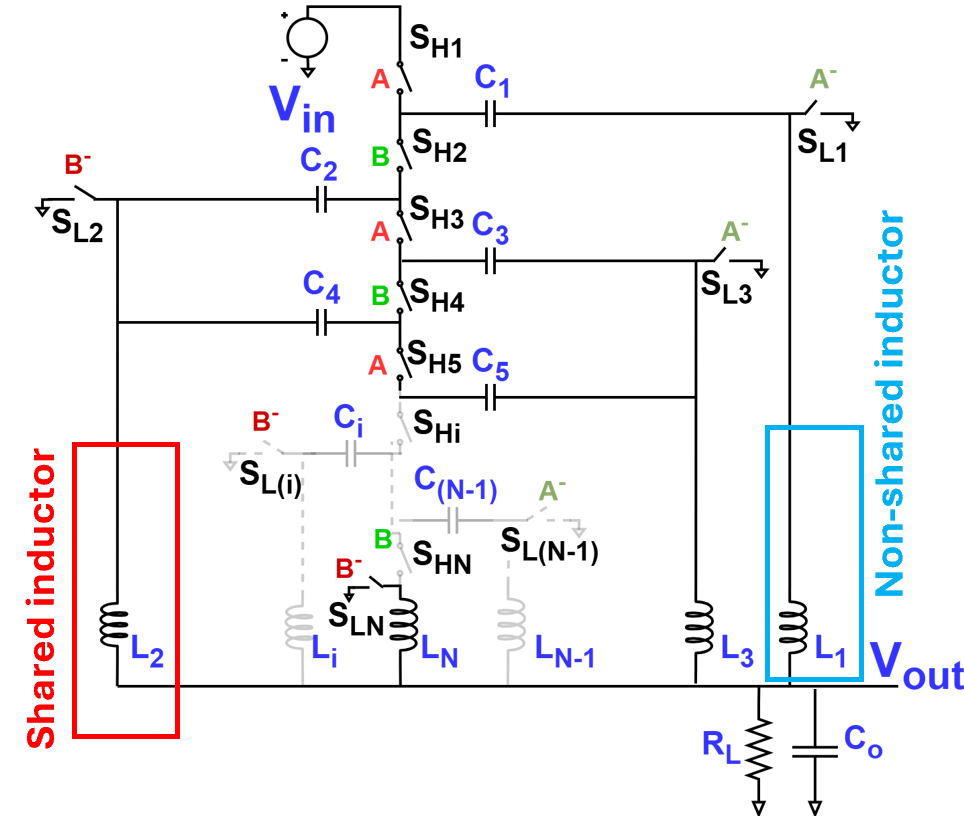
\includegraphics[width=0.39\textwidth]{HVR.png}
    \vspace{-5pt}
    \caption{Abstracted hybrid SC-buck regulator' topology.}
    \vspace{-5pt}
    \label{HVR}
\end{figure}

\subsection{SC-Buck HVR Topology}
The generalized SC-Buck HVR is shown in Fig.~\ref{HVR}. 
The input voltage is reduced to $V_{\mathrm{in}}/N$ by the
$N$ SC
branches and ${N}{-}1$ flying capacitors, lowering the HS switch voltage stress by a factor of
$N$. The use of low-voltage devices is thereby enabled, reducing switching
losses. The downstream buck stage comprises $K$ inductors,
each fed by $B_i \geq 1$ SC branches and commutating in one
of two interleaved phases (${K_A}$ in phase~A,
$K_\mathrm{B} = K - K_\mathrm{A}$ in phase~B). The SC-buck coupling is fully defined by the 
branch-assignment vector $\mathbf{B} = [B\mathrm{_1},\ldots,B\mathrm{_K}]$. The framework enumerates all valid
$({N},\,{K},\,\mathbf{B})$ combinations within the
user-defined constraints.

\vspace{-3pt}
\subsection{Analytical Loss Model}


The total HVR loss is
${\mathrm{P_{tot}} = \mathrm{P_{cond}} + \mathrm{P_{sw}^{HS}}
+ \mathrm{P_{sw}^{GD}} + \mathrm{P_{sw}^{OSS}}}$, where all terms
share the duty cycle $\mathrm{D} = \mathrm{NV_{out}/V_{in}}$, (identical across $K$ inductors since each switching
node swings between 0 and $V_\mathrm{in}/N$\cite{ECTCSal}).
Table~\ref{tab:loss} summarizes all expressions.
\vspace{-15pt}
\begin{table}[b]
%\renewcommand{\arraystretch}{1.8}
\caption{HVR Analytical Loss Model Equations.}
\label{tab:loss}
\centering
\scriptsize
\setlength{\tabcolsep}{5pt}
\begin{tabular}{|l|p{5.9cm}|}
\hline
\textbf{Term} & \textbf{Expression} \\
\hline
\textbf{Duty cycle} &
$\rule{0pt}{4ex}\mathrm{D} = {\mathrm{N}\,\mathrm{V_{out}}} / {\mathrm{V_{in}}}$ \\[5pt]
\hline

\textbf{RMS current} &
$\rule{0pt}{5ex}\mathrm{I_{load}^{rms}} = \sqrt{\mathrm{I_{load}^{2}}
  + \dfrac{\mathrm{D}^{2}
    \!\left(\tfrac{1}{\mathrm{N}}\mathrm{V_{in}}\mathrm{K_A}
    - \mathrm{V_{out}}\mathrm{K}\right)^{2}}
    {12\,\mathrm{f_{sw}}^{2}\mathrm{L}^{2}}}$ \\[5pt]
\hline

\textbf{Current ripple} &
$\rule{0pt}{4ex}\Delta\mathrm{I_{load}} = \dfrac{\mathrm{D}}{\mathrm{f_{sw}}\,\mathrm{L}}
  \!\left(\tfrac{1}{\mathrm{N}}\mathrm{V_{in}}\mathrm{K_A}
  - \mathrm{V_{out}}\mathrm{K}\right)$ \\[5pt]
\hline

\textbf{Conduction} &
$\rule{0pt}{4ex}\mathrm{P_{cond}} = \dfrac{\mathrm{V_{out}}}{\mathrm{V_{in}}}
  \,\mathrm{{I_{load}^{rms}}^{2}}\,\Omega_\mathrm{cond}$ \\[5pt]

& $\Omega_\mathrm{cond} = \mathrm{R_{HS}}
  + 2\!\left(1 - \tfrac{1}{\mathrm{N}}\right)\!\mathrm{R_C} 
  - \tfrac{1}{\mathrm{N}}(4\mathrm{B_k} - 1)\,\mathrm{R_{LS}}$\\[3pt]

& $\phantom{\Omega_\mathrm{cond} = {}}
  + \!\left[\dfrac{\mathrm{V_{in}}(\mathrm{R_L} + \mathrm{R_{LS}})}
               {\mathrm{N}^{2}\mathrm{V_{out}}}
  + \dfrac{2\,\mathrm{R_{LS}}}{\mathrm{N}}\right]
  \!\sum_{k}\mathrm{B}_i^{2}$ \\[5pt]

%& $\phantom{\Omega_\mathrm{cond} = {}}
%  - \dfrac{(4\mathrm{B_k} - 1)\,\mathrm{R_{LS}}}{\mathrm{N}}$ \\[2pt]
\hline

\textbf{HS switching} &
$\rule{0pt}{4ex}\mathrm{P_{sw}^{HS}} = \mathrm{f_{sw}}
  \!\left(\dfrac{\mathrm{V_{in}}}{\mathrm{N}} - \mathrm{V_{out}}\right)
  \!\mathrm{I_{load}^{rms}}
  \,\dfrac{\mathrm{Q_{GD}}}{\mathrm{I_g}}$ \\[3pt]

& $\mathrm{I_g} = \dfrac{\mathrm{V_{gs}}
    - \tfrac{1}{2}(\mathrm{V_{th}} + \mathrm{V_{pl}})}
    {\mathrm{R_{g,int}} + \mathrm{R_{drv}}}$ \\[4pt]
\hline

\textbf{Gate drive} &
$\mathrm{P_{sw}^{GD}} = \mathrm{f_{sw}}
  \!\left(\mathrm{N}\,\mathrm{Q_G^{HS}}
  + \mathrm{K}\,\mathrm{Q_G^{LS}}\right)
  \!\mathrm{V_{gs}}$ \\[3pt]
\hline

\textbf{Output Cap.\ loss} &
$\rule{0pt}{4ex}\mathrm{P_{sw}^{OSS}} =
  \dfrac{\mathrm{f_{sw}}}{2}
  (\mathrm{N C_{OSS}^{HS}} + \mathrm{K C_{OSS}^{LS}})\
  \!\left(\dfrac{\mathrm{V_{in}}}{\mathrm{N}}\right)^{\!2}$ \\[3pt]
\hline

\multicolumn{2}{|p{8.0cm}|}{%
  \scriptsize
  $\mathrm{R_{HS/LS}}$: FET on-resistance; $\mathrm{R_C}$: Cap.\ ESR; $\mathrm{R_L}$: Inductor DCR; $\mathrm{Q_{GD}}$: Miller charge; $\mathrm{Q_G}$: Total gate charge; $\mathrm{C_{OSS}}$: Output capacitance.%
  }\\
\hline
\end{tabular}
\end{table}





\subsection{Framework Overview}
As shown in Fig.~\ref{HVR_framework}, the framework enumerates all
valid HVR architectures, co-optimizes devices, passives, and switching
frequency via the closed-form loss model, and enforces all feasibility
constraints, outputting only physically realizable, minimum-loss
designs for any user-defined system inputs.

\begin{figure}[t]
    \centering
    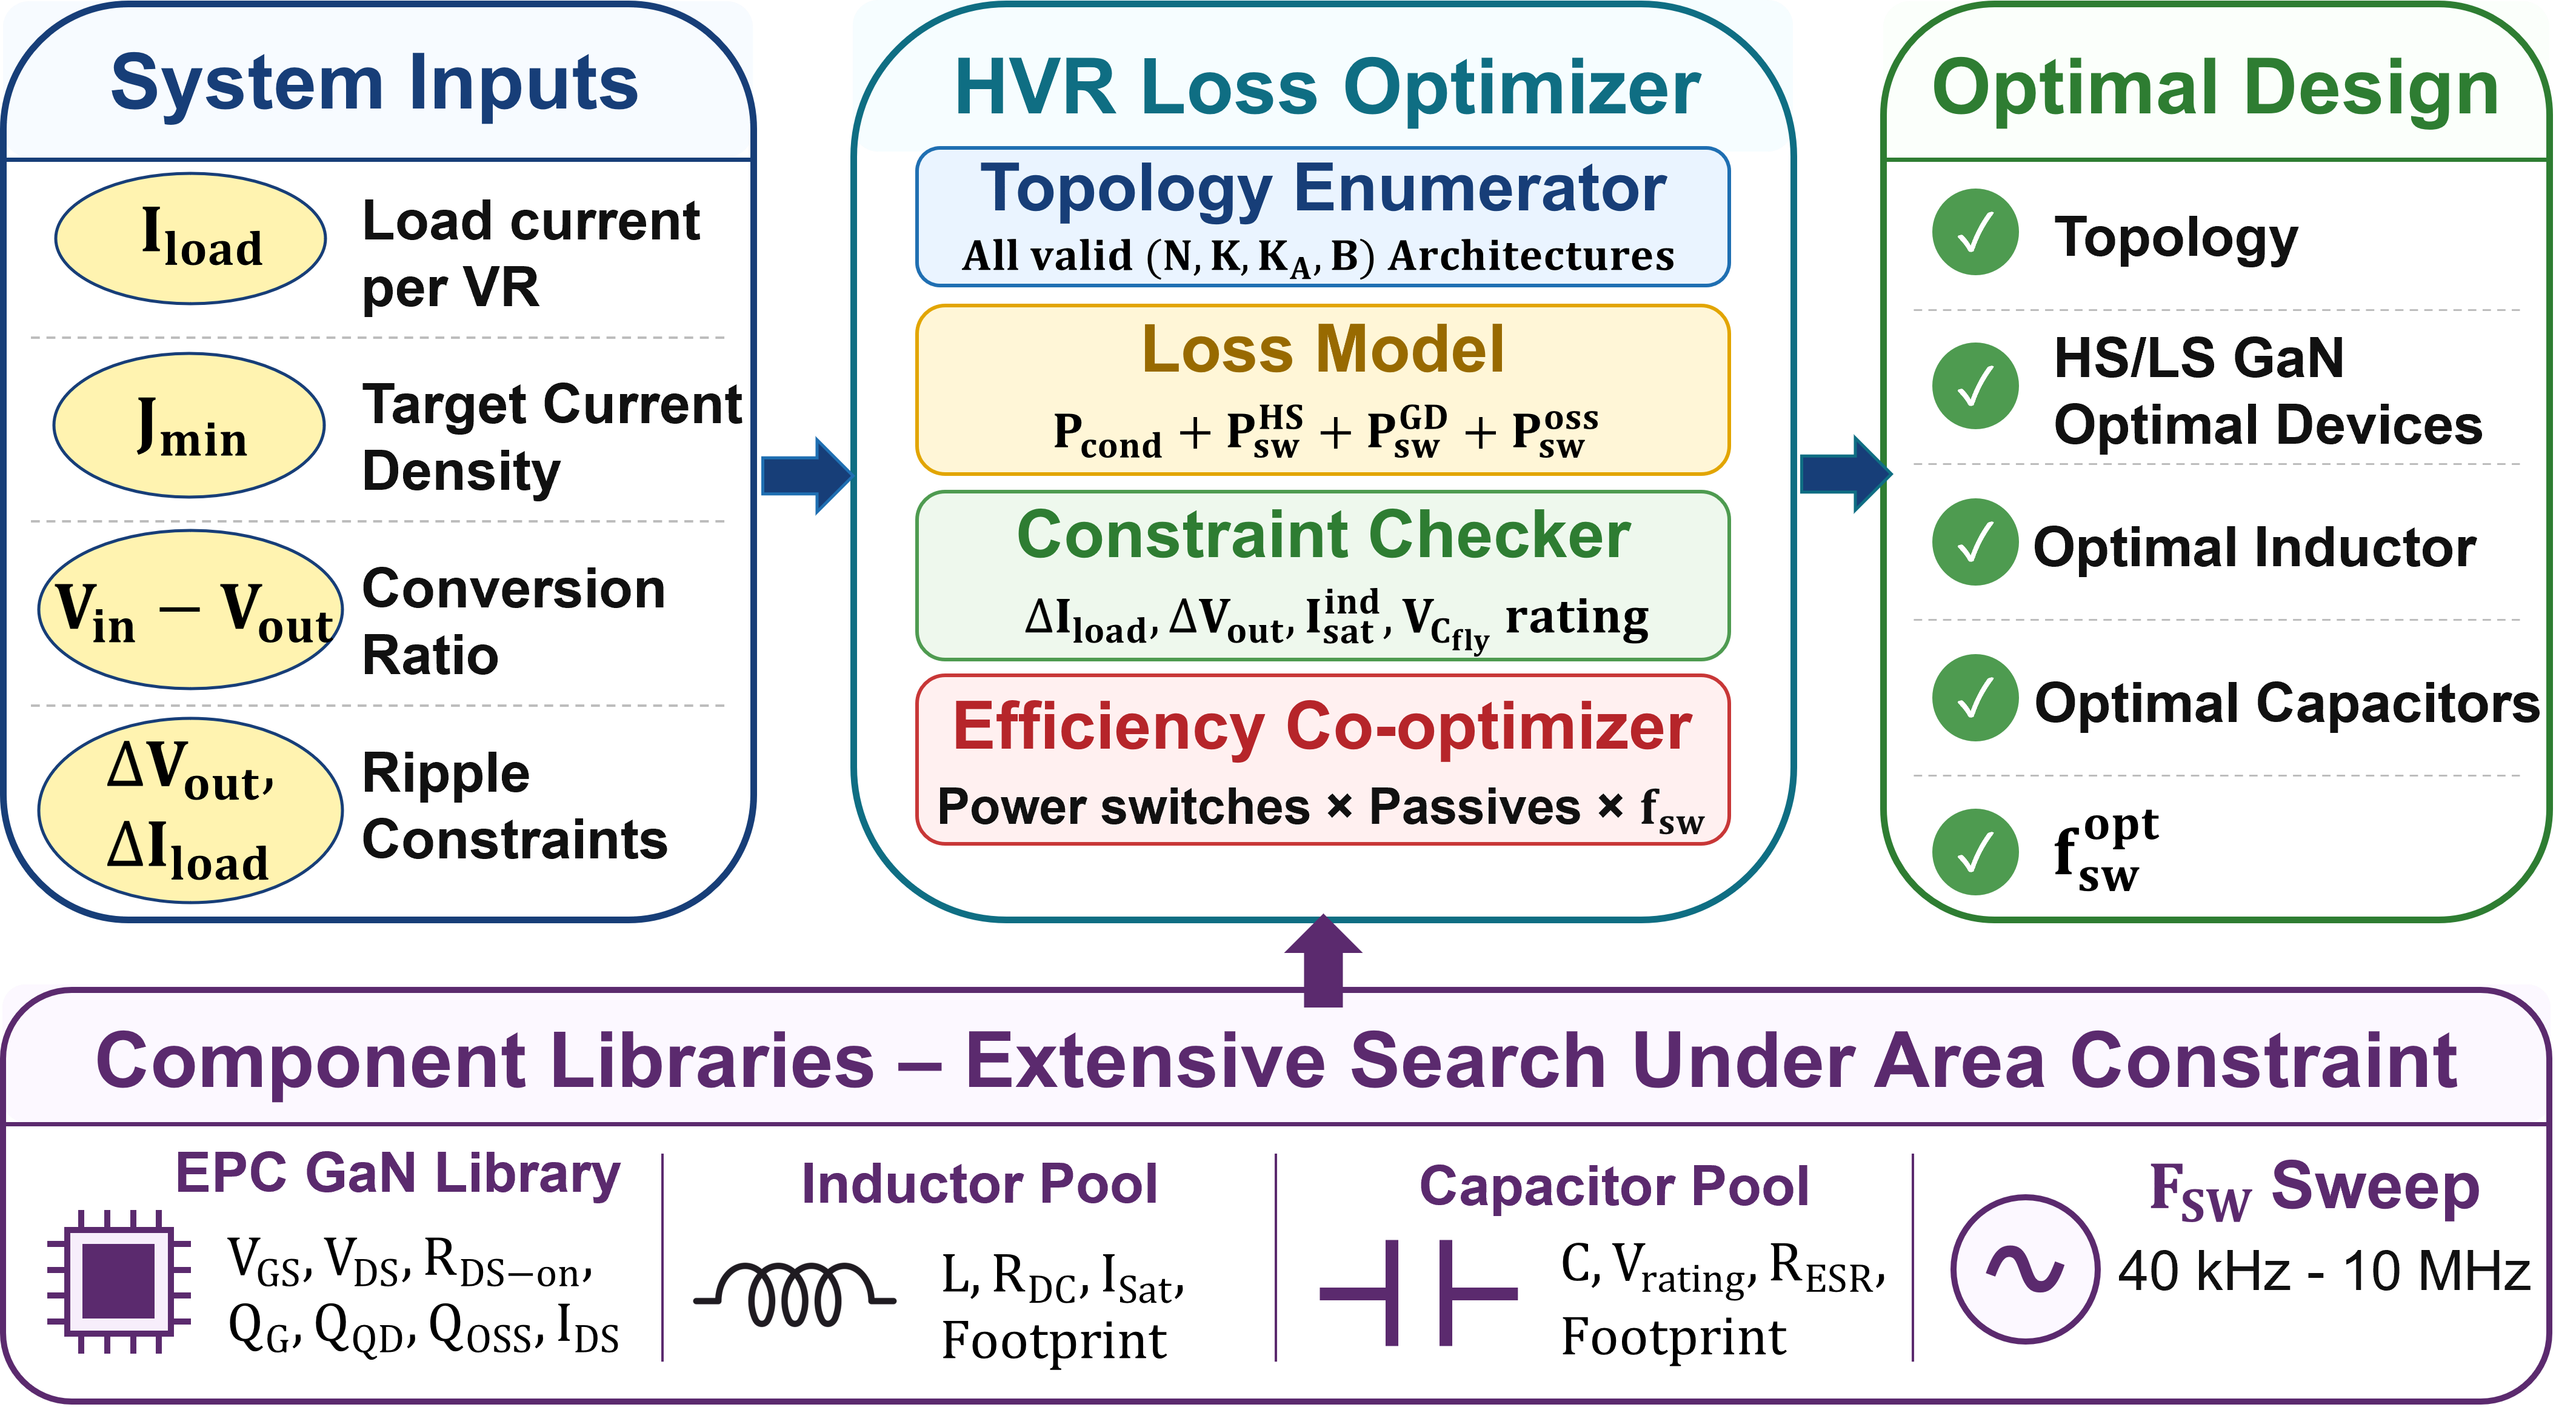
\includegraphics[width=0.48\textwidth]{HVR_framework_white.png}
    \caption{Proposed HVR optimization framework.}
    \vspace{-10pt}
    \label{HVR_framework}
\end{figure}




\section{Framework Output and Results Discussion}
\label{Framework output}

\subsection{Loss Model Validation}

Four SOTA topologies~\cite{DSCH, DPMIH44, DSCB, DPMIH62} are implemented
in Cadence Virtuoso/Spectre at 48~V-to-1~V, 30~A, 500~kHz with identical
EPC2216/EPC2014C switches, 3.3~\textmu F/3~m$\Omega$ capacitors, and
440~nH/0.21~m$\Omega$ inductors. As shown in Fig.~\ref{model_accuracy},
\textbf{95.27\%\,$\pm$\,1\%} mean loss prediction accuracy is achieved,
confirming model fidelity for DSE and optimization.
Note that these dominant loss mechanisms are sufficient for architecture-level DSE, while higher-order effects can be incorporated in future refinements.
\begin{figure}[h]
    \centering
    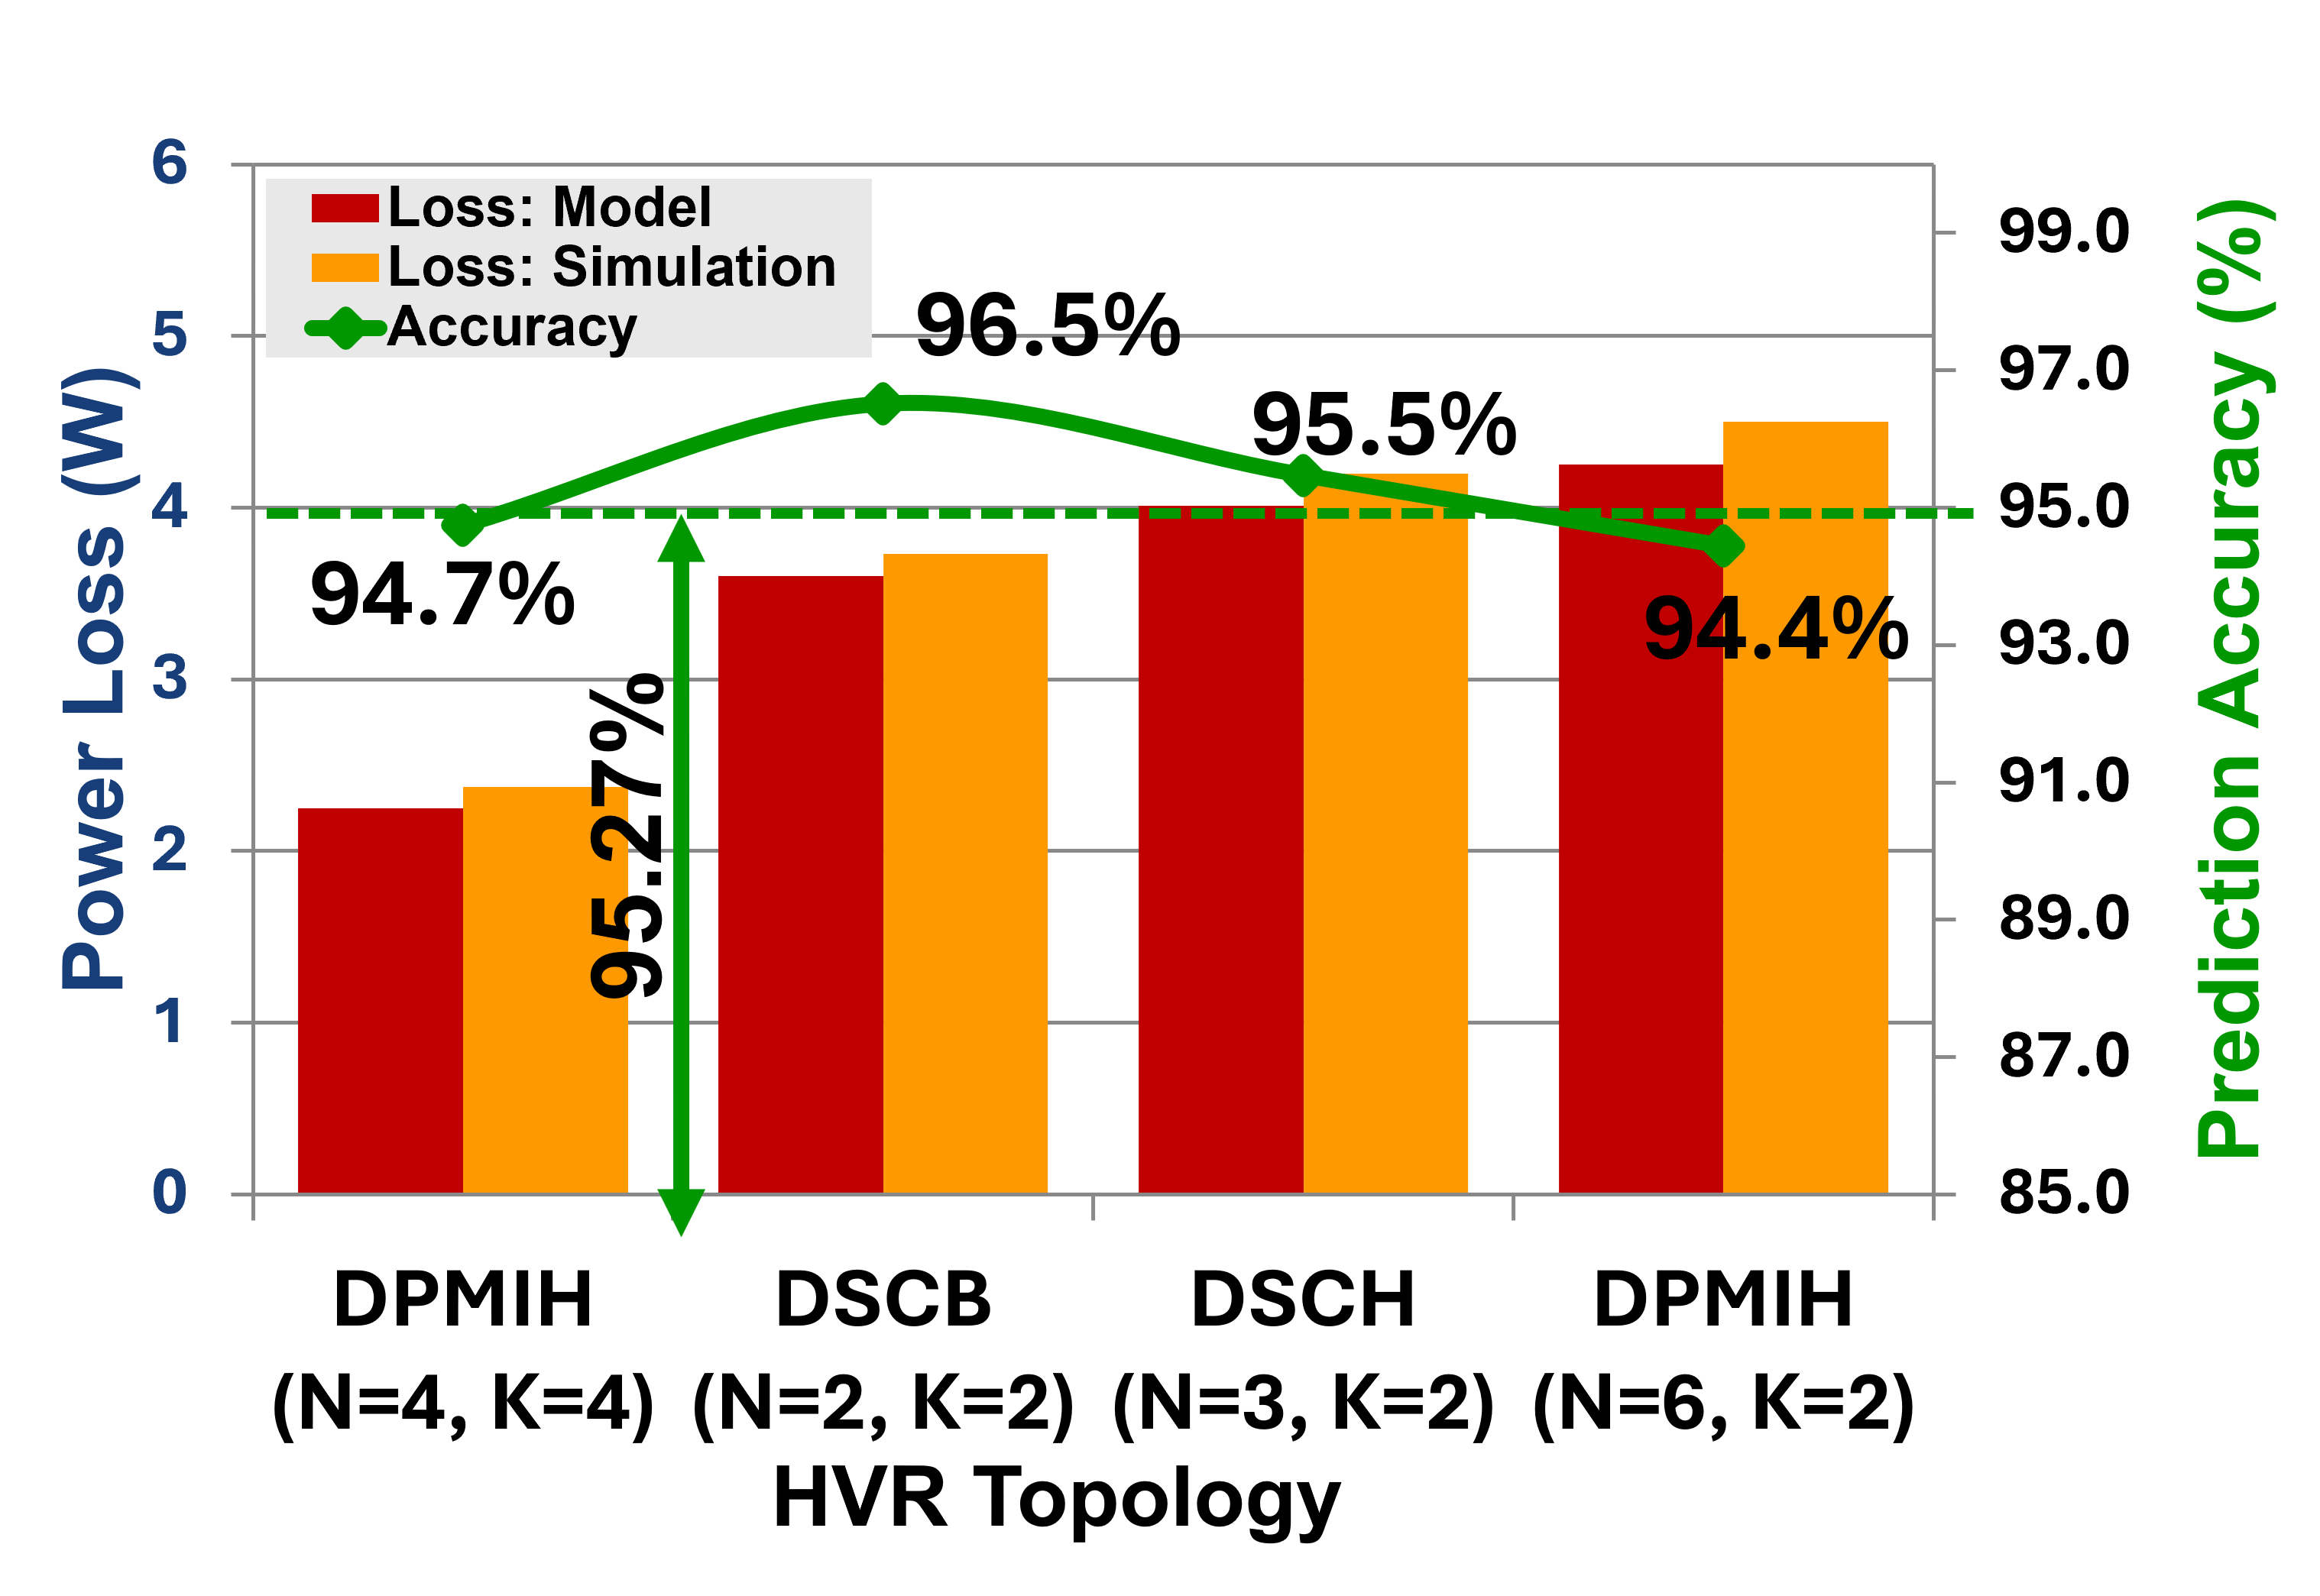
\includegraphics[width=0.45\textwidth]{Model_Accuracy_fixed.png}
    \caption{Loss model accuracy vs. simulation.}
    \vspace{-10pt}
    \label{model_accuracy}
\end{figure}

\subsection{Framework Comparison Against SOTA Designs}
For a fair comparison, the reported SOTA designs are first re-evaluated using the proposed
analytical loss model and their published component parameters, rather
than comparing directly against the reported experimental efficiencies.


Using this common baseline, the optimizer
identifies EPC2055/EPC2366 at 205~kHz for DSCH at 20~A, improving the routing lossless model efficiency from 93.1\% to 97.7\% (\textbf{+4.6~percentage points}), while reducing the footprint from 139.2 to 38.1~mm$^2$ ($3.7\times$), as shown in Table~\ref{tab:comparison}. For DPMIH at 25~A, a
\textbf{+2.7~percentage points} gain and $29\times$ footprint reduction are achieved.
Because the optimal frequency (328~kHz) closely matches the reported design (333~kHz),
this gain is attributed primarily to device selection. 
%Together, these results confirm that efficiency headroom and footprint savings unattainable by manual design are recovered by the framework.
These results demonstrate that systematic topology and component co-optimization uncovers substantial efficiency and footprint improvements beyond manually designed state-of-the-art implementations.

\begin{table}[t]
\renewcommand{\arraystretch}{1.45}
\caption{SOTA vs.\ Model-Driven Optimizer: Efficiency, Footprint, 
and Current Density}
\label{tab:comparison}
\centering
\scriptsize
\setlength{\tabcolsep}{2pt}
\begin{tabular}{|l|c|c|c|c|}
\hline

\textbf{Metric} 
  & \multicolumn{2}{c|}{\textbf{DSCH (N=3, K=2), 20~A}} 
  & \multicolumn{2}{c|}{\textbf{DPMIH (N=4, K=4), 25~A}} \\
\cline{2-5}

  & \textbf{SOTA \cite{DSCH}} & \textbf{Optimized} 
  & \textbf{SOTA \cite{DPMIH44}} & \textbf{Optimized} \\
\hline

\textbf{HS device} 
  &  Si4288DY & EPC2055 
  & 2$\times$EPC2015C & EPC2055 \\
\hline

\textbf{LS device} 
  & SiRA12DP & EPC2366 
  & 2$\times$EPC2023  & EPC2366 \\
\hline

\textbf{Switching frequency (kHz)} 
  & 500 & \textbf{205} 
  & 333 & \textbf{328} \\
\hline

\textbf{Footprint (mm$^2$)} 
  & 139.2 & \textbf{38.1} 
  & 2012.2  & \textbf{69.0} \\
\hline

\textbf{Current density (A/mm$^2$)} 
  & 0.14 & \textbf{0.52} 
  & 0.012 & \textbf{0.36} \\
\hline

\textbf{Efficiency\ (measured, \%)} 
  & 89.0~\cite{DSCH} & --- 
  & 91.5~\cite{DPMIH44} & --- \\
\hline

\textbf{Efficiency\ (modeled, \%)} 
  & 93.1\textsuperscript{a} & \textbf{97.7} 
  & 95.1\textsuperscript{b} & \textbf{97.8} \\
\hline


\textbf{Efficiency gain (pp)} 
  & \multicolumn{2}{c|}{\textbf{+4.6}} 
  & \multicolumn{2}{c|}{\textbf{+2.7}} \\
\hline


\textbf{Footprint reduction} 
  & \multicolumn{2}{c|}{\textbf{3.7$\times$ smaller}} 
  & \multicolumn{2}{c|}{\textbf{29.2$\times$ smaller}} \\
\hline
\end{tabular}
%\vspace{2pt}

\begin{flushleft}
    \scriptsize 
    \textsuperscript{a}Estimated device-specific routing loss: 4.1\%\\
    \textsuperscript{b}Estimated device-specific routing loss: 4.4\%
\end{flushleft}
\vspace{-15pt}
\end{table}

\subsection{Packaging-Aware Design-Space Exploration}

DSE capability is demonstrated through a 48~V-to-1~V, 20~A case study
under a 20~mm$^2$ budget (1~A/mm$^2$) with $\Delta\mathrm{I} < 40\%$
and $\Delta\mathrm{V} < 5\%$ ripple constraints, for two packaging
scenarios. \textbf{Case~1}: planar 2D integration where HVR area is determined by the sum of all component footprints; \textbf{Case~2}: 3D
vertical stacking where HVR area is constrained by the footprint of the largest component.
As shown in Figs.~\ref{case_planar}--\ref{case_stacked}, all feasible
SC-buck topologies are enumerated and co-optimized over device and
passive libraries, with the minimum-loss implementation reported for each topology. Current and Voltage-ripple utilization remain below 100\% for all reported designs, confirming constraint satisfaction.

In Case~1, N=3, K=2 is optimal at 97.0\%; the
planar budget restricts high-$K$ topologies to smaller, higher-resistance devices, degrading conduction efficiency.
In Case~2, vertical stacking relaxes the area constraints, enabling larger, lower-resistance devices and shifting the optimum to N=4, K=2 at 97.4\%. Every topology
outperforms its Case~1 counterpart, confirming that vertical
integration improves efficiency even at \emph{identical} current
density. For any $V_\mathrm{in}:V_\mathrm{out}$, load, and packaging
constraints, the optimal topology, devices, passives, and switching frequency
are autonomously identified, enabling systematic package-aware design-space exploration without exhaustive manual optimization.


\begin{figure}[t]
    \centering
    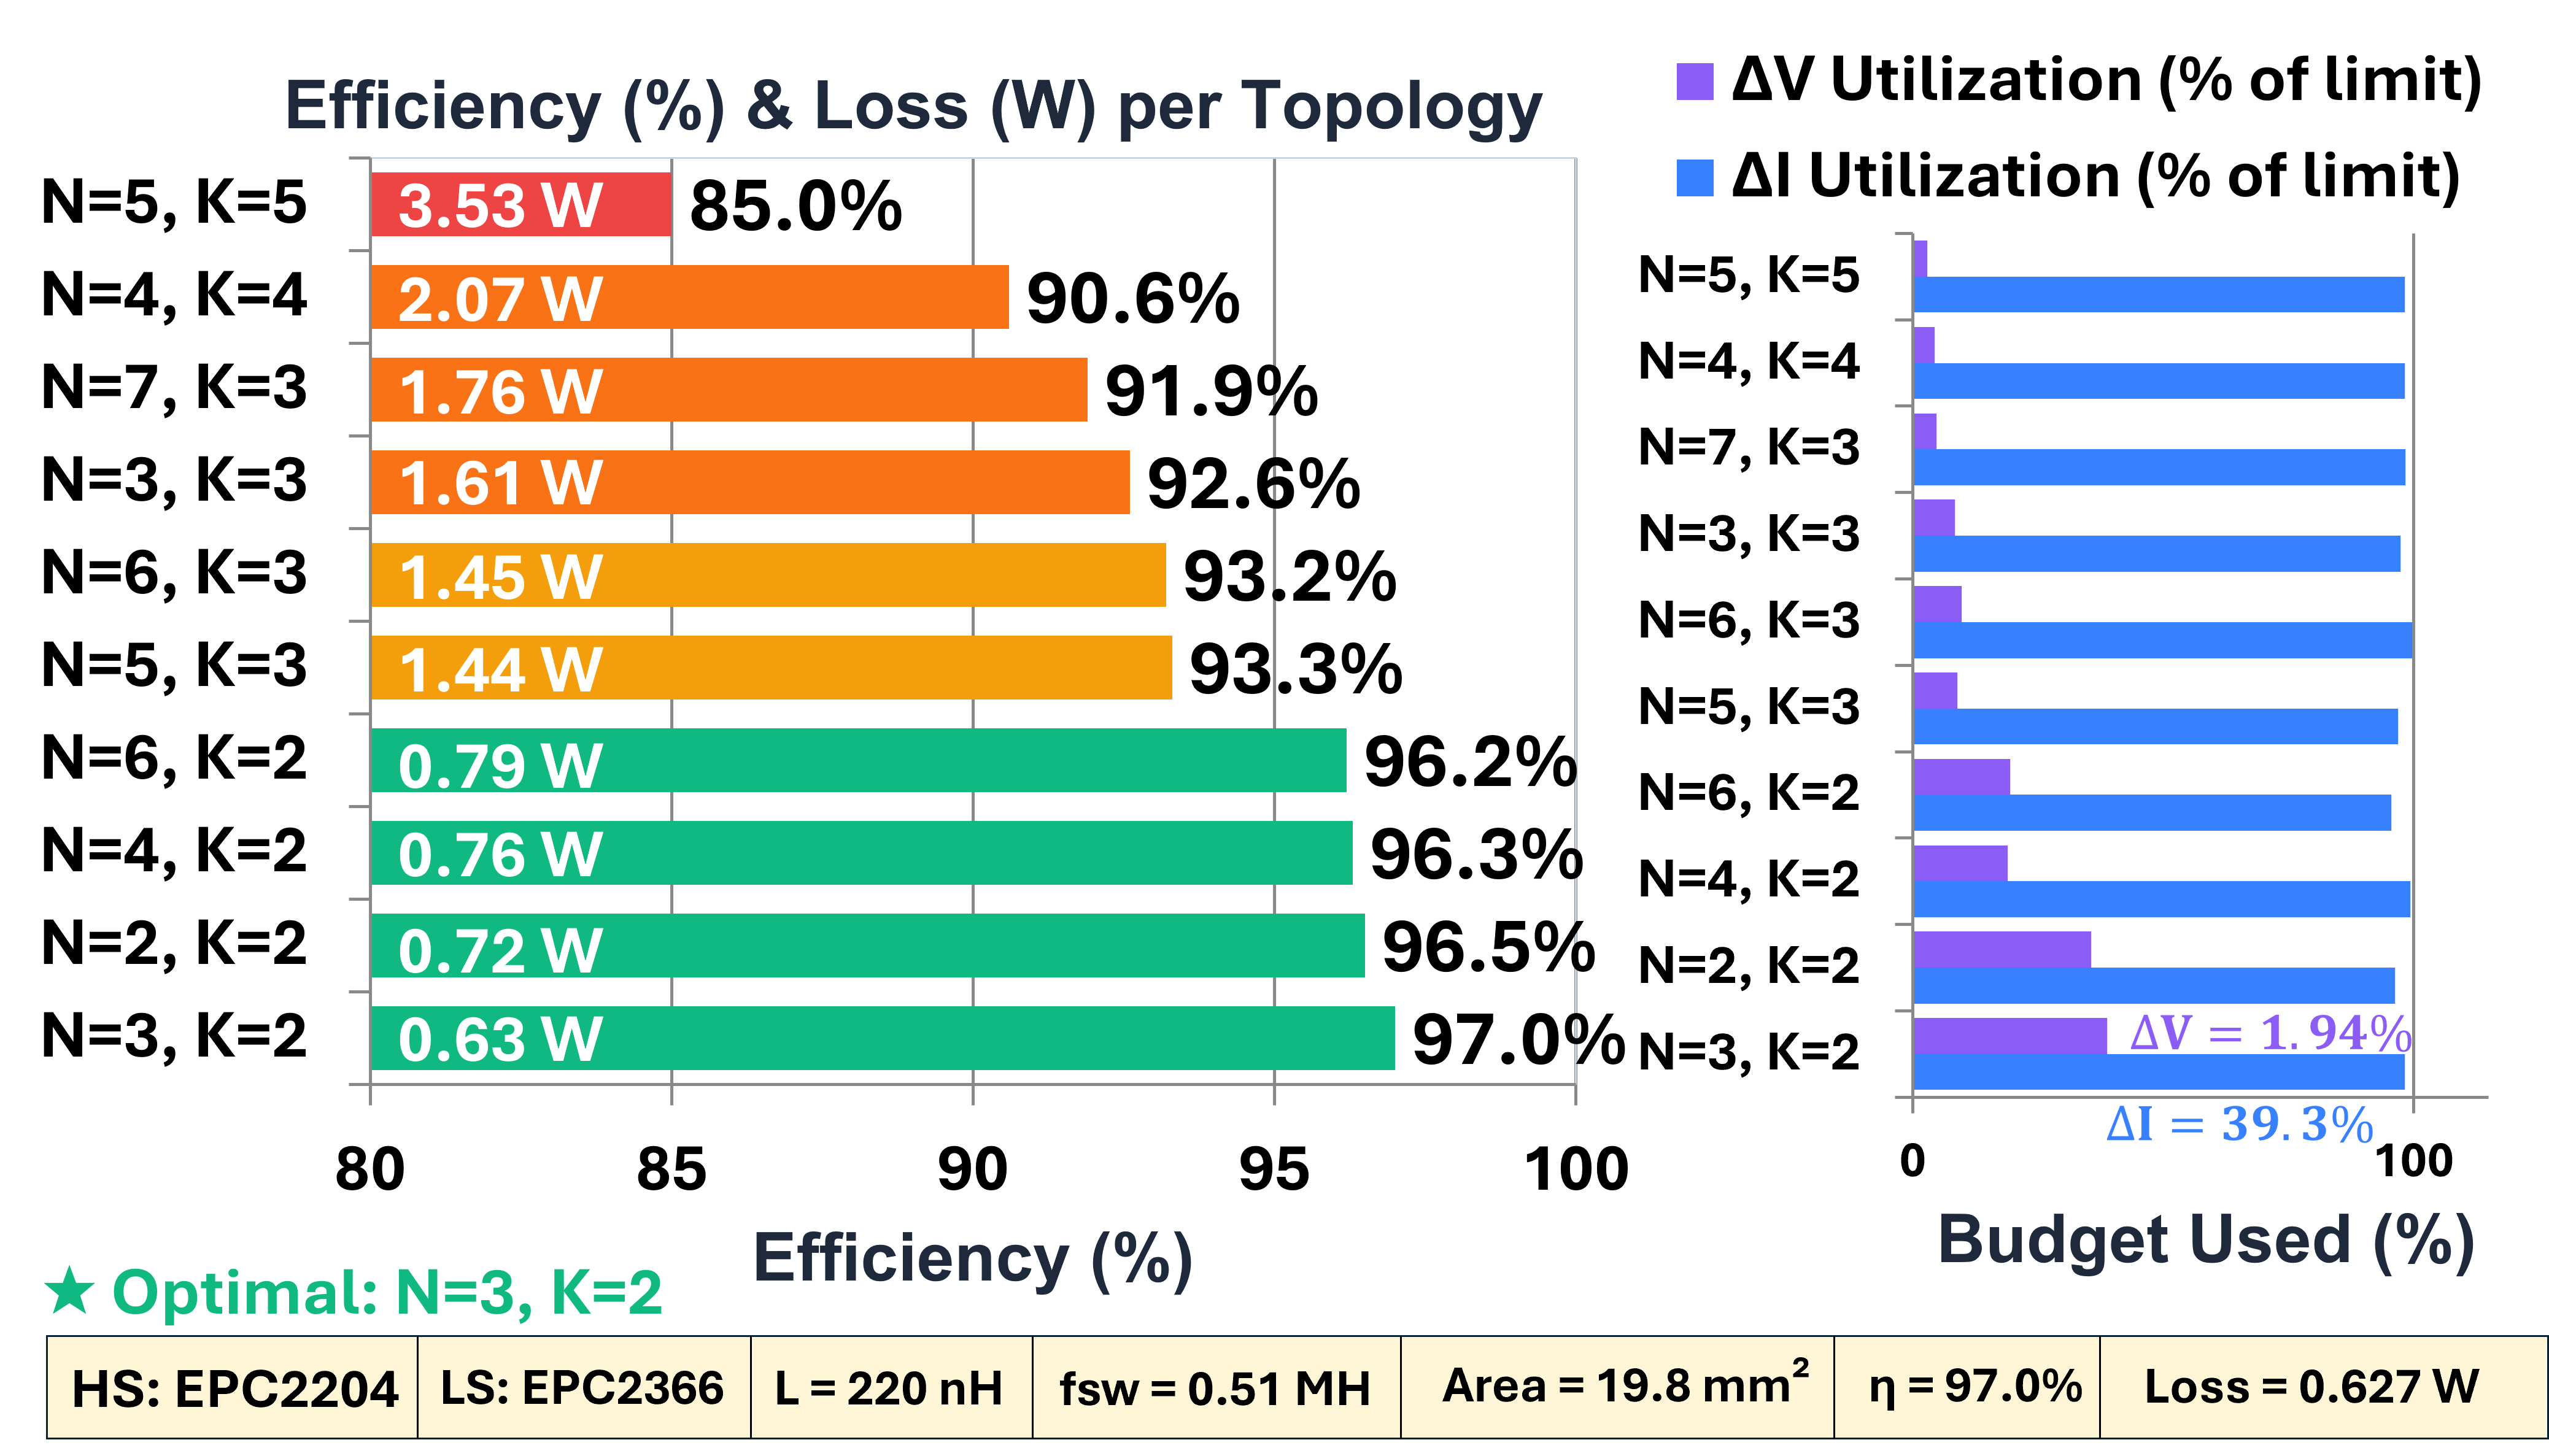
\includegraphics[width=0.48\textwidth]{case_planar.png}
    \caption{DSE for 2D planar HVR integration (Case 1).}
    \vspace{-10pt}
    \label{case_planar}
\end{figure}

\begin{figure}[h]
    \centering
    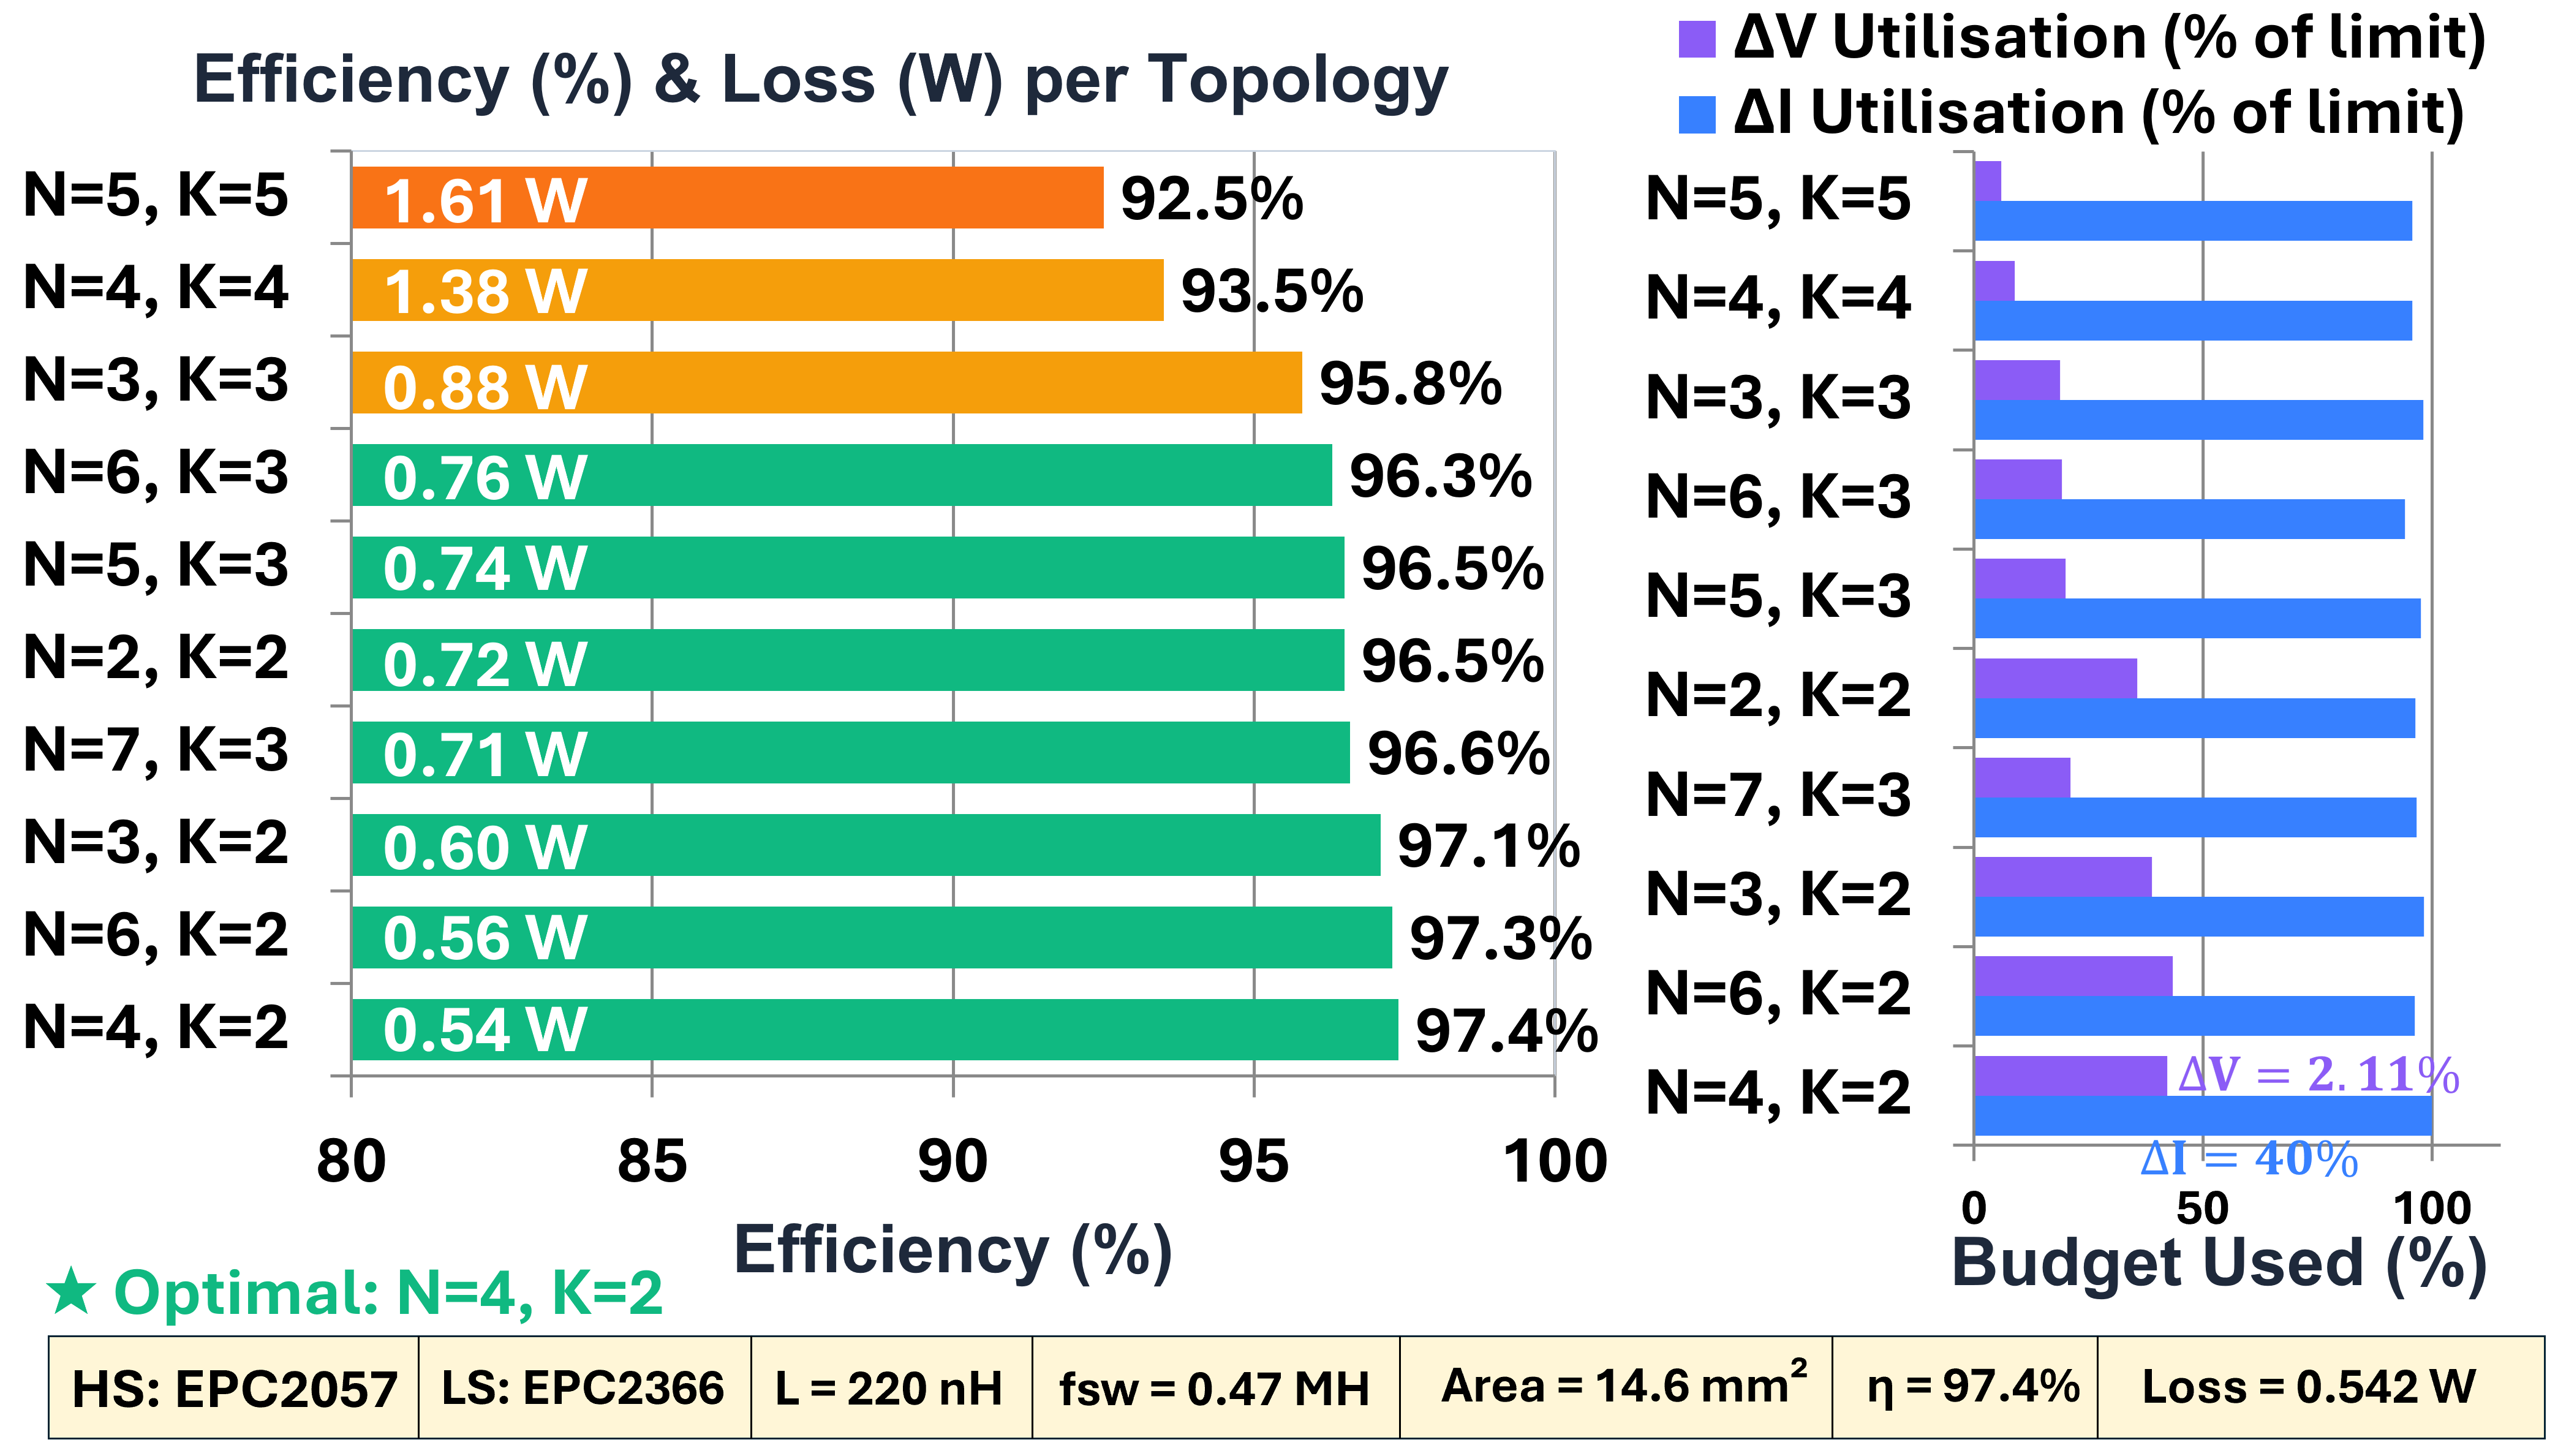
\includegraphics[width=0.48\textwidth]{case_stacked.png}
    \caption{DSE for HVR integration with vertical stacking (Case 2).}
    \vspace{-15pt}
    \label{case_stacked}
\end{figure}


\section{Conclusion}
A packaging-aware DSE framework for SC-buck HVRs is presented, targeting high-step-down vertical power delivery for AI data centers. Feasible topologies are enumerated and co-optimized over discrete power switches, passives, and switching frequency under electrical and footprint constraints using a closed-form loss model. At 95.27\%$\pm$1\% mean accuracy against Spectre simulations, up to \textbf{+4.6~pp} efficiency improvement and \textbf{29.2$\times$}
footprint reduction over state-of-the-art implementations are achieved. The results further demonstrate that the optimal HVR topology depends on the integration scheme, establishing circuit--package co-optimization as a key requirement for next-generation AI data-center POL design.





\bibliography{References}
\bibliographystyle{ieeetr}


\end{document}
